%%==========================
%% chapter01.tex for SJTU Master Thesis
%% based on CASthesis
%% modified by wei.jianwen@gmail.com
%% version: 0.3a
%% Encoding: UTF-8
%% last update: Dec 5th, 2010
%%==================================================

%\bibliographystyle{sjtu2} %[此处用于每章都生产参考文献]
\chapter{核心技术和内存计算框架}
\label{chap:FFTandCos}

傅里叶变换是一种线性的积分变换\upcite{bracewell1980fourier}。其算法思想首先由法国学者傅里叶系统地提出,所以以他的名字来命名以示纪念。傅里叶变换在很多领域中都有广泛的应用,比如物理学,光学,量子力学,组合数学等等,它的典型用途是将信号分解成振幅分量和频率分量。

傅里叶变换一共有四种变体,它们分别是连续傅里叶变换、傅里叶级数、离散时间傅里叶变换、离散傅里叶变换,如图\ref{fig:type}所示。对于非周期性连续信号,通常使用傅里叶变换;对于周期性连续信号,通常使用傅里叶级数;对于非周期性离散信号,通常使用离散时域傅里叶变换;对于周期性离散信号,通常使用离散傅里叶变换。在这四种变体中,本文主要关注离散傅里叶变换以及它的另外一种计算方法,即快速傅里叶变换,在下一小节中将做详细的介绍。

\begin{figure}[!h]
\centering
    \begin{minipage}[b]{1\textwidth}
    \captionstyle{\centering}
    \centering
    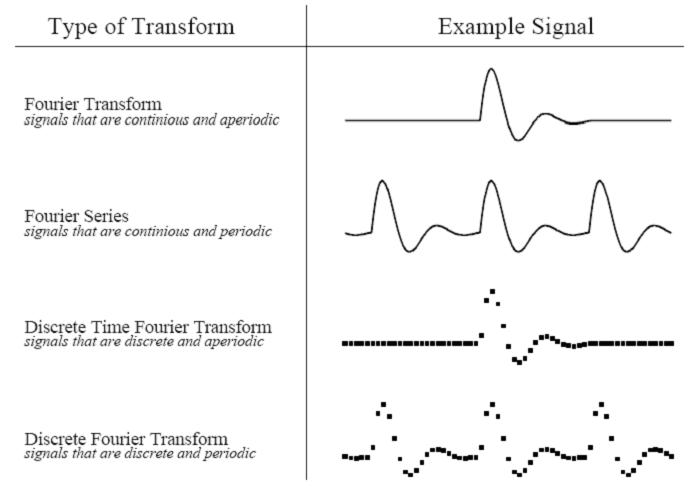
\includegraphics[origin=br,width=14cm]{chap3/typeOfFT.jpg}
    \bicaption[fig:type]{傅里叶变换种类}{傅里叶变换种类.}{Fig}{types of different fourier transform.}
    \end{minipage}     
\end{figure}
\section{快速傅里叶变换}
\label{sec:FT}

\subsection{离散傅里叶变换}
\label{sec:DFT}
什么是DFT(Discrete Fourier Transform)?简单来说,它是一种算法,接受的输入为一组离散的在时域上的信号,输出为信号在频域上的标示。在这个上下文中,信号指的是一串序列的数字。为了在科学计算和数字信号处理等领域使用离散傅里叶变换,$x_n$必须满足离散非连续,且有限或有周期。DFT的直观计算复杂度是$O(n^2)$,而快速傅里叶变换(FFT)可以把这个复杂度降低到$O(nlog(n))$,FFT将在下一小节中详细说明。

计算机为什么只能处理离散傅里叶变换?这是因为,在计算机的角度来看,它无法处理连续的信号,连续信号只有在数学推导的过程中才会用到。而对于非周期性离散信号,我们需要使用无穷多的不同频率的正弦或余弦曲线来表示,这对于计算机而言也是不可能办到的,所以对离散信号的变换只有DFT可以被适用。

\subsubsection{复数}
复数作为DFT的一种输入得到了广泛的用途和应用。复数是一种形式诸如$a+bi$的数,其中a和b都是实数,i被称为虚部,它满足$i^2=-1$。利用复数可以把由两个变量表达的式子由一个变量来表达,方便了之后的计算和表达。复数有很多种表达方法,比如上面提到的$a+bi$,一种更普遍的表达方式是用极坐标的方式。用复数表示正弦余弦表达式将非常地简洁和方便,比如下式的左边可以和右边互相转化$$A\cos (wt) + B\sin (wt) == a + bi$$在离散信号处理中,运用复数来解决问题是一个非常常用的技巧,对复数的各种运算和对原来的正弦余弦信号的处理结果是相同的,同时必须满足下列条件:

\begin{enumerate}
\item 所有参与运算的正弦波和余弦波的频率是一样的
\item 运算操作必须是线性的
\end{enumerate}

\subsubsection{复数形式的DFT}
傅里叶变换的输出是由两部分组成,使用复数可以可以缩减表达式,使得我们处理一个变量而非两个,而后面将介绍的FFT正式基于复数的,所以大多数情况下的DFT的输入都是基于复数形式的。复数形式的DFT使得DFT变得更加简洁。DFT的正向变换等式为:$$X(k)=\frac{1}{N}\sum_{n=0}^{N-1}x(n)(\cos(\frac{2\pi kn}{N}) - j\sin(\frac{2\pi kn}{N}))$$

这个式子经过欧拉变换以后可以得到:$$X(k)=\frac{1}{N}\sum_{n=0}^{N-1}x(n)e^{\frac{-j2\pi kn}{N}}$$

\subsection{快速傅里叶变换}
\label{sec:FFT}

在1965年,库利和图基发表了一篇论文,首次提出了DFT运算的一种快速形式,即Fast fourier transform(FFT)\upcite{walker1996fast}。FFT用了一些小技巧做了和DFT相同的事情,但是大大减小的运算时间。

FFT算法的基本思想,就是利用周期和对称性,并且将长序列分为短序列,大大减少DFT中的计算量。本章节主要介绍FFT中的一些算法设计要点,如下:

\begin{enumerate}
\item 将长度为N的时域序列$x_n$按奇偶分为两部分,记其中一个$n/2$个点的DFT为$x_1(k)$,记另一个$n/2$个点的DFT为$x_2(k)$
\item 可以推导出原序列前$n/2$个点的DFT为$$X(k)=X_1(k)+W^k_NX_2(k)$$之后$n/2$个点的DFT则不需要计算,否则计算量并没有减少。考虑到周期性和对称性,利用前一半的运算结果,可以用来计算后一半的值,这种算法被叫做蝶形算法,通过推导可以看出,用这种算法的计算量比普通的DFT的计算量少了约一半。
\item 如果把时间序列二分为四,长度均为$n/4$,反复使用蝶形算法,计算量可以在原来的基础上再减小一半。以此类推,直到把长度为n的序列分解成$n/2$个2点运算,计算量就可以大大减小。通过对这个算法求算法复杂度可知,这个算法的复杂度为$O(nlog(n))$
\end{enumerate}

那么这个速度大概可以提高多少倍呢,假设$n=4096$,DFT将计算1677万次,而FFT只需要4.9万次,提升了300多倍,这是一个相当巨大的提升。

由上面的分析可知,FFT大大地减少了DFT在数字信号处理中的运算量,使得很多很复杂的信号可以得到快速的处理,这项算法的发明具有里程碑的意义。本文将利用快速傅里叶变换作为本文提出的算法核心中关键的一步,关于本文算法的设计将在后面几个章节中详细说明。

\section{N维向量相似度计算技术}

余弦定理在数学上是用来计算两个N维向量夹角的算法。本节将说明为什么余弦定理可以用来检测相似度。想象有两个N维向量,若他们是完全相同的,那么他们的余弦值就为1,即夹角为0°,此时说明他们完全相同;若有任意一个N维向量的某一维发生了改变,改变得越大,余弦值越偏离1,夹角越偏离0°,此时他们可能是相似文件,要看这个上下文种对相似是怎么定义的,比如当余弦夹角$\theta$小于一个预设的值$\epsilon$,则表示这两个N维向量是相似的。本文将在算法设计上采用类似的思想。

该定理早在2006年的时候就被谷歌用在了新闻的分类上。所谓新闻的分类就是把相似的新闻放在一类。计算机读不懂新闻,计算机只知道快速运算,所以谷歌的做法是像一篇新闻报道做预处理,输出为一个N维向量,这里N的取值为常用词汇的总量,第$x$维的值等于这个词汇的TF/IDF值,如果某个词汇没有在文章新闻中出现,那么TF/IDF的值就为0,经过这样的变换,可以将新闻转化为一个N维的向量,作为这篇新闻的特征向量,如果两个特征向量的夹角非常小,那么我们就可以认为这两篇新闻是类似的。

由于某些原因,余弦定理的应用场景会受到一些限制,在后文中将讨论这种限制以及一些可能的解决方法。

\section{基于内存计算的框架}
\label{sec:framework}
在本小节中,将主要介绍和研究在当今互联网大数据环境下的计算框架和模型,将详细讨论hadoop和spark这两种较为主流的框架,它们之间的异同点,以及优缺点和计算效率问题。

\subsection{Apache Hadoop}
Hadoop\upcite{white2009hadoop}是一个开源的软件框架为了存储和在集群上的大规模数据的处理。整个Hadoop框架由以下四个方面构成:

\begin{enumerate}
\item Hadoop Common - 提供其它Hadoop模块需要的库和功能
\item Hadoop Distributed File System (HDFS)\upcite{shvachko2010hadoop} - 一个分布式文件系统
\item Hadoop YARN - 一个资源管理的平台
\item Hadoop MapReduce - 一个为大型数据处理设计的编程模型
\end{enumerate}
hadoop有很高的容错性,硬件可能随时宕机,然而框架保证了从错误中的及时恢复。Hadoop MapReduce和HDFS最初的是来源于Google MapReduce和Google File System。下面简单讨论以下hadoop的整体架构。一个小型的hadoop集群有一个master节点和若干个worker节点组成;master节点由Jobtracker, TaskTracker, NameNode和DataNode组成;一个worker由DataN
ode和taskTracker组成。在一个大集群中,HDFS由一个特殊的NameNode来管理,类似的,一个单独的Jobtracker来管理任务分配。

HDFS是hadoop框架下的一个分布式的,可拓展的文件系统。大量的dataNode组成了HDFS集群。节点和节点之间通过TCP/IP协议来进行通信。HDFS在不同的机器之间存储存储大型文件(从几G到几T的大小)。它是用重复存储来保证数据的可靠性,默认情况下是每个文件存储三份拷贝,所以就可以不需要使用RAID。HDFS中有一个叫做secondary namenode,它的作用是定期连接primary namenode做快照的功能,这些检查点可以被用来重启一个失败primary namenode。使用HDFS的一个好处是在jobTracker和taskTracker之间能够知道数据在哪个节点。比如,jobTracker将要分配一个map任务的时候,发现A节点处有数据X,B节点处有数据Y,那么A节点就会被调度在数据X做map任务,B节点就会被调度在数据Y做map任务,这就避免了不必要的网络数据的传输,其它的文件系统不一定会有如此的优势。

在HDFS之上架着MapReduce引擎,它由一个jobTracker构成,用户态的应用程序向它提交MapReduce任务。JobTracker将任务分给可用的TaskTracker,使得数据的移动代价最小。JobTracker知道数据存储在哪些节点上,并且也知道哪些节点离数据最近。如果一个TaskTracker失败或者超时了,这个task就会被重新分配。TaskTracker会每隔几分钟发一个心跳给JobTracker来检查状态。关于调度方法,一共有两种较为主流的方法:

\begin{enumerate}
\item Fair scheduler

由Facebook首次提出,这个调度的目的是为了小任务提供较快的相应时间和为了对生产任务提供QoS。
\item Capacity scheduler

由Yahoo首次提出,它支持的若干特性和Fail scheduler差不多,此处不详细展开。
\end{enumerate}

Hadoop被广泛用在工业界处理当今互联网形式下大数据,它的最大的几个用户包括雅虎,Facebook等。2010年,Facebook声称他们拥有世界上最大的hadoop集群,有着21PB的数据量,在2013年,他们又声称数据量已经增长到了100PB。

\subsection{Apache Spark}
虽然hadoop在大数据处理上应用广泛,但仍由一些更加优秀的平台逐渐产生。
Spark\upcite{zaharia2010spark}是一个快速的通用的集群计算系统,它提供了高层的Scala,Java,Python的API来使得并行任务容易写,在它之上有许多高层的应用,比如Shark,MLlib,GraphX,这些和本文关系不大,将不详细讨论。
Spark融合了内存计算,相对于Hadoop的集群存储,性能上更具优势。Spark最核心的概念是RDD(Resilient Distributed Dataset),在Spark以前的计算系统中,基本上都是基于非循环的数据流模型,也就是说每一次计算都必须经历外存中读取,然后计算,最后写回外存的整个过程,这样的模型使得那些使用重复数据的运算无法高效进行,于是spark就在这样的环境下诞生。

RDD的设立理念是保留类似MapReduce这样的框架优点的同时,使得可以将一部分数据集保存在内存中供加速之后的查询和计算。在容错机制上,RDD使用了记录更新着这种方法作为主要方法
\section{小结}
\label{sec:conc}

本章详细介绍了下一章节中提出算法中的关键技术和概念,快速傅里叶变换(FFT)和向量相似度的比较基数。傅里叶变换是一种线性的积分变换,其算法思想首先由法国学者傅里叶系统地提出,所以以他的名字来命名以示纪念。傅里叶变换在很多领域中都有广泛的应用,比如物理学,光学,量子力学,组合数学等等,它的典型用途是将信号分解成振幅分量和频率分量。而余弦定理作为一种非常强大的工具也有非常跨领域的应用,特别是在2006年被谷歌用在了新闻的分类上。本章讨论的各种技术将为主要算法章节做铺垫。
